\documentclass[11pt]{article}
\usepackage{geometry}
\geometry{letterpaper, margin=1in}
\usepackage{graphicx}
\usepackage{listings}
\usepackage{xcolor}
\usepackage[utf8]{inputenc}
\usepackage[T1]{fontenc}
\usepackage{lmodern}
\usepackage{float}
\usepackage{booktabs}
\usepackage{tabularx}
\usepackage{amsmath}
\usepackage{tikz}
\usepackage{pgfplots}
\usepackage{pgfplotstable}
\usepackage{hyperref}

\usetikzlibrary{arrows.meta, positioning, shapes.geometric, calc}
\pgfplotsset{compat=1.18}

\lstset{
    basicstyle=\ttfamily\small,
    breaklines=true,
    frame=single,
    showstringspaces=false,
    language=C++
}

% Screenshots live in ./screenshots
\graphicspath{{screenshots/}}

% \screenshot{file}{caption}{label}
% Shows screenshots/<file> if it exists; otherwise a placeholder box so the
% report still compiles before the screenshots are added.
\newcommand{\screenshot}[3]{%
  \begin{figure}[H]
    \centering
    \IfFileExists{screenshots/#1}{%
      \includegraphics[width=\textwidth,height=0.42\textheight,keepaspectratio]{#1}%
    }{%
      \fbox{\parbox[c][3cm][c]{0.9\textwidth}{\centering
        \textbf{Screenshot missing}\\[4pt]
        Save it as \texttt{report/screenshots/\detokenize{#1}}}}%
    }
    \caption{#2}
    \label{#3}
  \end{figure}}

\newcommand{\question}[2]{\subsection*{Question #1}\noindent\textit{#2}\par\medskip}
\newcommand{\code}[1]{\texttt{#1}}

% Numbers and tables below come from ./lab --experiment (make data)
% Generated by ./lab --experiment. Do not edit by hand.
\newcommand{\FaultRateFits}{0.51}
\newcommand{\FaultRateDouble}{50.43}
\newcommand{\FaultRateQuad}{75.12}
\newcommand{\DistinctPages}{541}
\newcommand{\MetricAddresses}{1000}
\newcommand{\MetricHitRate}{4.30}
\newcommand{\MetricHits}{43}
\newcommand{\MetricFreeFaults}{263}
\newcommand{\MetricFaults}{544}
\newcommand{\MetricEvictions}{281}
\newcommand{\MetricInvalidations}{7}
\newcommand{\MetricCycles}{192.40}
\newcommand{\MetricPageTables}{257}
\newcommand{\TwoLevelKB}{2072}
\newcommand{\FlatKB}{8192}
\newcommand{\MinHitRate}{4.30}
\newcommand{\MaxHitRate}{4.40}
\newcommand{\AvgHitRate}{4.31}
\newcommand{\AvgFaults}{545.5}
\newcommand{\AvgCycles}{192.38}
\newcommand{\BaseCycles}{200.00}
\newcommand{\LocalHitRate}{89.14}
\newcommand{\LocalCycles}{22.71}
\newcommand{\LocalBaseCycles}{200.00}
\newcommand{\TimeTLB}{0.0592}
\newcommand{\TimeNoTLB}{0.0301}
\newcommand{\LocalTimeTLB}{0.0304}
\newcommand{\LocalTimeNoTLB}{0.0174}

\pgfplotstableread[col sep=comma]{data/tlb_size.csv}\tlbsizetable
\pgfplotstableread[col sep=comma]{data/working_set.csv}\workingsettable

% Chart colors and style
\definecolor{seriesblue}{HTML}{2A78D6}
\definecolor{seriesorange}{HTML}{EB6834}
\definecolor{chartink}{HTML}{52514E}
\definecolor{chartgrid}{HTML}{E1E0D9}
\definecolor{chartaxis}{HTML}{C3C2B7}
\pgfplotsset{
  labchart/.style={
    width=0.82\textwidth, height=6cm,
    axis lines=left, axis line style={chartaxis, -},
    ymajorgrids, major grid style={solid, line width=0.3pt, chartgrid},
    tick style={draw=none},
    tick label style={font=\sffamily\footnotesize, text=chartink},
    label style={font=\sffamily\footnotesize, text=chartink},
    legend style={draw=none, fill=none, font=\sffamily\footnotesize, text=chartink,
                  at={(0.5,1.03)}, anchor=south, legend columns=-1, column sep=6pt},
    legend cell align=left,
    clip=false,
  },
  blueline/.style={seriesblue, line width=1.2pt, mark=*, mark size=2.2pt,
                   mark options={fill=seriesblue, draw=white, line width=0.5pt}},
  orangeline/.style={seriesorange, line width=1.2pt, mark=square*, mark size=2.1pt,
                     mark options={fill=seriesorange, draw=white, line width=0.5pt}},
}

% Diagram styles
\tikzset{
  endlabel/.style={font=\sffamily\footnotesize, text=chartink, anchor=west, xshift=3pt},
  box/.style={draw=chartink, rectangle, minimum height=7mm, align=center, font=\small},
  entry/.style={draw=chartink, rectangle, minimum width=22mm, minimum height=5.5mm,
                font=\footnotesize\ttfamily},
  flow/.style={-{Stealth[length=2mm]}, chartink, line width=0.6pt},
  flowstep/.style={box, rounded corners=2pt, minimum width=38mm, text width=36mm, fill=white},
  choice/.style={draw=chartink, diamond, aspect=2.2, inner sep=1pt, align=center,
                 font=\small, fill=white},
}

\begin{document}
\sloppy

\title{CS-375 Operating Systems Lab 8:\\Caching, TLB, and Multi-level Page Tables}
\author{Santiago Soto}
\date{\today}
\maketitle

\tableofcontents
\newpage

%=====================================================================
\section{Design Overview}

The simulator in \code{main.cpp} translates 32-bit virtual addresses with 4\,KB
pages. Each part of the lab is a mode of the same program, chosen with
\code{-{}-part}, and Part 4 is the default.

\begin{table}[H]
\centering
\begin{tabularx}{\textwidth}{clX}
\toprule
\textbf{Part} & \textbf{Command} & \textbf{What runs} \\
\midrule
1 & \code{./lab -{}-part 1} & Direct-mapped table with $2^{20}$ entries. \\
2 & \code{./lab -{}-part 2} & 2-level table, created on demand. \\
3 & \code{./lab -{}-part 3} & 2-level table with a 16-entry LRU TLB. \\
4 & \code{./lab} & Part 3 limited to 256 frames, with random invalidation and eviction. \\
\bottomrule
\end{tabularx}
\caption{Modes of the simulator.}
\end{table}

\subsection{2-Level Page Table}

A virtual address splits into a 10-bit directory index, a 10-bit table index and
a 12-bit offset. The directory has 1024 entries, each pointing to a second-level
table of 1024 entries, which gives $1024 \times 1024 = 2^{20}$ virtual pages.
Second-level tables are allocated only when a region is first used.

\begin{figure}[H]
\centering
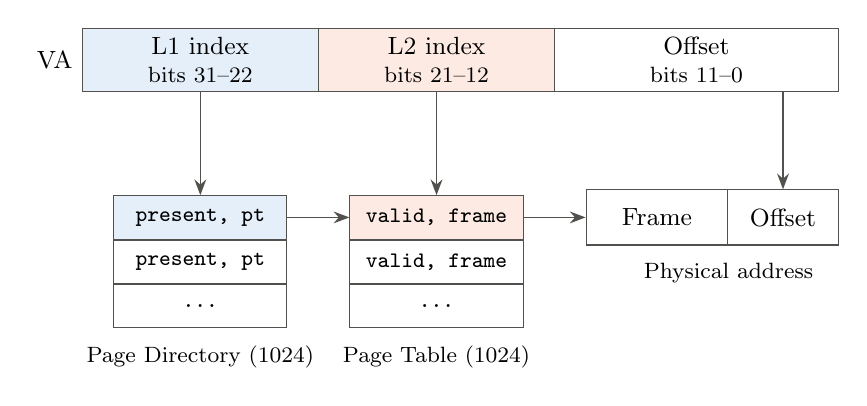
\begin{tikzpicture}
  % Address fields
  \node[left, font=\small] at (0,0) {VA};
  \node[box, minimum width=30mm, fill=seriesblue!12] (l1) at (1.5,0) {L1 index\\[-1pt]\footnotesize bits 31--22};
  \node[box, minimum width=30mm, fill=seriesorange!14] (l2) at (4.5,0) {L2 index\\[-1pt]\footnotesize bits 21--12};
  \node[box, minimum width=36mm] (off) at (7.8,0) {Offset\\[-1pt]\footnotesize bits 11--0};

  % Page directory
  \node[entry, fill=seriesblue!12] (pd0) at (1.5,-2) {present, pt};
  \node[entry, below=0mm of pd0] (pd1) {present, pt};
  \node[entry, below=0mm of pd1] (pd2) {\dots};
  \node[below=1mm of pd2, font=\footnotesize] {Page Directory (1024)};

  % Page table
  \node[entry, fill=seriesorange!14] (pt0) at (4.5,-2) {valid, frame};
  \node[entry, below=0mm of pt0] (pt1) {valid, frame};
  \node[entry, below=0mm of pt1] (pt2) {\dots};
  \node[below=1mm of pt2, font=\footnotesize] {Page Table (1024)};

  % Physical address
  \node[box, minimum width=18mm, minimum height=7mm] (frame) at (7.3,-2) {Frame};
  \node[box, minimum width=14mm, minimum height=7mm] (poff) at (8.9,-2) {Offset};
  \node[below=1mm of frame.south east, font=\footnotesize] {Physical address};

  \draw[flow] (l1) -- (pd0);
  \draw[flow] (l2) -- (pt0);
  \draw[flow] (pd0) -- (pt0);
  \draw[flow] (pt0) -- (frame);
  \draw[flow] (poff.north |- off.south) -- (poff);
\end{tikzpicture}
\caption{The two lookups of a page table walk. The L1 index selects a directory
entry, which points to a page table. The L2 index selects the page table entry,
which holds the frame. The offset is copied unchanged.}
\label{fig:two-level}
\end{figure}

\subsection{TLB Structure and LRU Logic}

The TLB is fully associative with 16 entries. Each entry stores \code{vpn},
\code{pfn}, \code{timestamp} and \code{valid}, and any page can sit in any entry.
A lookup compares the VPN with every valid entry. The TLB keeps a clock that
increases on every lookup hit and every insert, and that access stamps the entry
with the new clock value. The entry with the smallest timestamp is therefore the
least recently used, and it is replaced on insert. An empty slot has timestamp 0,
so it is always filled before a live entry is replaced.

\subsection{Flowchart: VA to PA}

\begin{figure}[H]
\centering
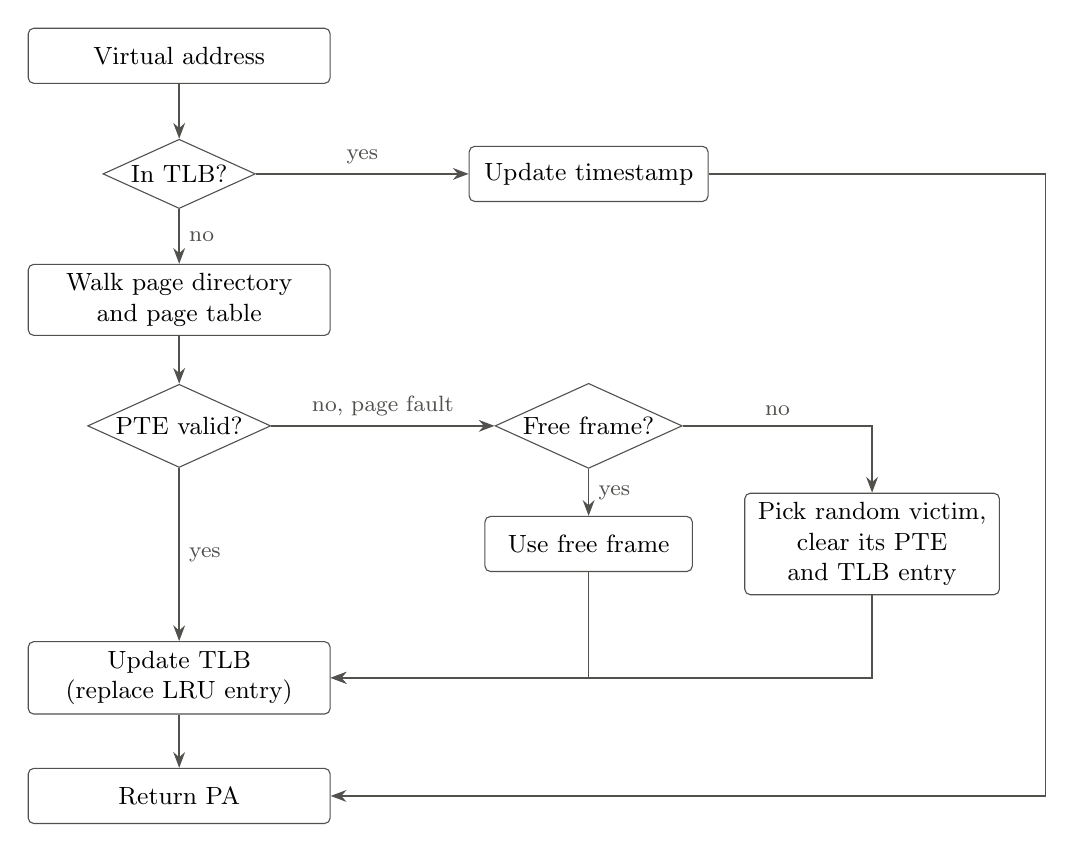
\begin{tikzpicture}
  % Main path
  \node[flowstep] (va) at (0,0) {Virtual address};
  \node[choice] (hit) at (0,-1.5) {In TLB?};
  \node[flowstep] (walk) at (0,-3.1) {Walk page directory\\and page table};
  \node[choice] (valid) at (0,-4.7) {PTE valid?};
  \node[flowstep] (update) at (0,-7.9) {Update TLB\\(replace LRU entry)};
  \node[flowstep] (pa) at (0,-9.4) {Return PA};

  % TLB hit and page fault paths
  \node[flowstep, minimum width=30mm, text width=28mm] (stamp) at (5.2,-1.5) {Update timestamp};
  \node[choice] (free) at (5.2,-4.7) {Free frame?};
  \node[flowstep, minimum width=26mm, text width=24mm] (take) at (5.2,-6.2) {Use free frame};
  \node[flowstep, minimum width=32mm, text width=30mm] (evict) at (8.8,-6.2) {Pick random victim, clear its PTE and TLB entry};

  \draw[flow] (va) -- (hit);
  \draw[flow] (hit) -- node[right, font=\footnotesize] {no} (walk);
  \draw[flow] (walk) -- (valid);
  \draw[flow] (valid) -- node[right, font=\footnotesize] {yes} (update);
  \draw[flow] (update) -- (pa);
  \draw[flow] (hit) -- node[above, font=\footnotesize] {yes} (stamp);
  \draw[flow] (stamp.east) -| (11,-9.4) -- (pa.east);
  \draw[flow] (valid) -- node[above, font=\footnotesize] {no, page fault} (free);
  \draw[flow] (free) -- node[right, font=\footnotesize] {yes} (take);
  \draw[flow] (free.east) -| node[pos=0.25, above, font=\footnotesize] {no} (evict.north);
  \draw[flow] (take.south) |- (update.east);
  \draw[flow] (evict.south) |- (update.east);
\end{tikzpicture}
\caption{Translation flow in Part 4.}
\label{fig:flow}
\end{figure}

%=====================================================================
\section{Implementation Highlights}

\subsection{How Page Faults Are Simulated}

Part 4 allows only 256 frames. Three lists track physical memory:
\code{free\_frames}, \code{allocated\_frames}, and \code{frame\_owner}, which maps
each frame back to the VPN stored in it.

A fault happens when a walk finds an invalid page table entry, either on the
first access to a page or after the page lost its frame. Pages lose their frames
in two ways:
\begin{itemize}
  \item \textbf{Random invalidation.} Before each access there is a 1\% chance
  that a random resident page is invalidated and its frame is freed. This stands
  in for the operating system reclaiming a page.
  \item \textbf{Eviction.} If a fault finds no free frame, a random allocated
  frame is chosen as the victim and its current page is removed.
\end{itemize}

Removing a page must clear both the page table entry and any TLB entry for that
page. Otherwise the TLB would keep sending the old page to a frame that now holds
different data.

\begin{lstlisting}
uint32_t allocate_frame(uint32_t vpn, bool& evicted) {
    uint32_t frame;
    evicted = free_frames.empty();
    if (evicted) {
        frame = allocated_frames[random_allocated_slot()];
        unmap_frame(frame);    // clears the PTE and the TLB entry
        stats.evictions++;
    } else {
        frame = free_frames.back();
        free_frames.pop_back();
        allocated_frames.push_back(frame);
    }
    frame_owner[frame] = vpn;
    return frame;
}
\end{lstlisting}

\subsection{LRU in the TLB (Timestamp Method)}

A hit refreshes the entry's timestamp, and an insert scans for the smallest one.
Both operations take $O(n)$ time in the number of entries, which is acceptable
for 16 entries.

\begin{lstlisting}
void insert(uint32_t vpn, uint32_t pfn) {
    size_t lru_idx = 0;
    uint64_t oldest = entries[0].timestamp;
    for (size_t i = 1; i < entries.size(); i++) {
        if (entries[i].timestamp < oldest) {
            oldest = entries[i].timestamp;
            lru_idx = i;
        }
    }
    entries[lru_idx].vpn = vpn;
    entries[lru_idx].pfn = pfn;
    entries[lru_idx].timestamp = ++clock;
    entries[lru_idx].valid = true;
}
\end{lstlisting}

The TLB holds its entries in a vector sized by a constructor argument instead of
a fixed \code{entries[16]} array. The default stays 16, and Section~\ref{sec:size}
uses the same class for 4, 8 and 32 entries.

\subsection{Changes from the Provided Skeleton}

The skeleton needed these corrections to complete the lab.

\begin{table}[H]
\centering
\begin{tabularx}{\textwidth}{XX}
\toprule
\textbf{Problem in the skeleton} & \textbf{Change} \\
\midrule
\code{allocate\_frame} loops forever once all 256 frames are used, and this trace
touches \DistinctPages{} pages. & Added eviction with a random victim. \\
Eviction did not exist, so nothing removed a page from the TLB. &
Added \code{TLB::invalidate}, called whenever a page loses its frame. \\
\code{fin >{}> hex >{}> addr} fails on \code{0x7fff5fbff000}, which is 48 bits wide,
and silently ends the input. & Each address is read as 64 bits. Wider addresses
print a warning and use their low 32 bits. \\
\code{hex} stays set on \code{cout}, so summary counts print in hexadecimal. &
Hexadecimal formatting is confined to a helper, \code{hex32}. \\
\code{make run} runs \code{./generate} without building it. &
\code{addresses.txt} is now a Makefile target that depends on \code{generate}. \\
Timing the printing loop measures terminal output rather than translation. &
Time is measured separately with printing off (Section~\ref{sec:perf}). \\
\bottomrule
\end{tabularx}
\caption{Corrections to the skeleton.}
\end{table}

Two details of the handout are also worth noting. Its example address
\code{0x7fff5fbff000} does not fit in a 32-bit address space, so the simulator
uses \code{0x5fbff000} and page \code{0x5fbff}. The comment in
\code{generate\_addresses.cpp} called the hot region 100 pages, but the range
\code{0x70000000} to \code{0x700FFFFF} is 1\,MB, which is 256 pages. The code
is unchanged and the comment is corrected.

%=====================================================================
\section{Screenshots}

\subsection{Build}
\screenshot{01_build.png}{Building the lab with the provided compiler flags.}{fig:build}

\subsection{Part 1: Direct-Mapped Page Table}
\screenshot{02_part1.png}{Part 1 on the handout's sample addresses, including the
warning for the 48-bit address.}{fig:part1}

The first address maps to physical address 0 as in the handout, because frames
are assigned in order on first use. Six addresses cause only 5 faults, since
\code{0x00001abc} and \code{0x00001def} are in the same page: both use the same
frame and keep their own offsets. Every translation costs 100 modeled cycles,
because a flat table needs one memory access.

\subsection{Part 2: 2-Level Page Table}
\screenshot{03_part2.png}{Part 2 summary, with page table memory compared to the
flat table.}{fig:part2}

Part 2 gives the same translations as Part 1 for the same addresses, but
the two designs trade time against space. The 2-level table costs 200 cycles per
translation, twice the flat table, because it needs two memory accesses. In
exchange it uses \TwoLevelKB{}\,KB instead of \FlatKB{}\,KB, because only
\MetricPageTables{} of the 1024 second-level tables were created. The saving is
modest here because random addresses touch many regions. A program with a compact
address space would need only a few tables.

\subsection{Part 3: TLB}
\screenshot{04_part3.png}{Part 3 TLB hits and summary.}{fig:part3}

Only \MetricHits{} of \MetricAddresses{} translations hit. All of them fall in the
first 700 addresses, where $43/700 = 6.1\%$ closely matches the 6.25\% expected from
16 entries covering 256 hot pages. The last 300 addresses never hit, because each
goes to a different page. The average cost matches the formula in
Section~\ref{sec:perf}: $1 + 0.957 \times 200 = \MetricCycles$ cycles.

\subsection{Terminal Output: First 10 and Last 10 Lines}
\screenshot{05_first_10.png}{First 10 lines of the Part 4 output.}{fig:first}

The run starts with empty memory, so the first accesses are all page faults that
take a free frame, followed by a TLB miss. Frame numbers look random because
Part 4 shuffles the free list.
\screenshot{06_last_10.png}{Last 10 lines of the Part 4 output, with the summary.}{fig:last}

By the end of the run memory is full, so faults evict a frame instead of taking a
free one.

\subsection{PAGE FAULT Messages}
\screenshot{07_page_faults.png}{Page faults that evicted a frame, and the total
number of faults.}{fig:faults}

The fault counts add up. The trace touches \DistinctPages{} distinct pages, so
that many faults were unavoidable, and the other few came from pages that were
invalidated or evicted and then used again. Of the \MetricFaults{} faults,
\MetricFreeFaults{} found a free frame: the 256 frames available at the start, plus
the \MetricInvalidations{} freed by random invalidation. The remaining
\MetricEvictions{} had to evict.

\subsection{TLB Hit Rate}
\screenshot{08_hit_rate.png}{TLB hit rate averaged over 10 random seeds.}{fig:hitrate}

The hit rate stays between \MinHitRate\% and \MaxHitRate\%, averaging
\AvgHitRate\%. The seed changes only which pages are invalidated and evicted, and
the address trace stays fixed. It also matches Part 3, which has no memory limit.
The first eviction happens at about address 716, after the last hit, so the frame
limit never removes a page that was about to hit.

\subsection{Without the TLB}
\screenshot{09_no_tlb.png}{The same run with the TLB turned off.}{fig:notlb}

The page fault count is unchanged, because a TLB only caches translations and has
no effect on which pages are in memory. The cost is exactly 200 cycles, since
every translation now walks the table.

%=====================================================================
\section{Performance Analysis}
\label{sec:perf}

\subsection{Summary Metrics}

These are the results for \code{addresses.txt} in the default Part 4
configuration with seed 42. Averages use seeds 42 to 51.

\begin{table}[H]
\centering
\begin{tabular}{lr}
\toprule
\textbf{Metric} & \textbf{Value} \\
\midrule
TLB Hit Rate & \MetricHitRate\% \\
TLB Hit Rate (average of 10 runs) & \AvgHitRate\% \\
Page Faults & \MetricFaults \\
Page Faults (average of 10 runs) & \AvgFaults \\
Evictions & \MetricEvictions \\
Random Invalidations & \MetricInvalidations \\
Avg Translation Time & \TimeTLB{} $\mu$s \\
Avg Translation Cost & \MetricCycles{} modeled cycles \\
\bottomrule
\end{tabular}
\caption{Summary metrics for \code{addresses.txt}.}
\end{table}

\textbf{Page faults.} The \MetricFaults{} faults are high for 1000 addresses
because the trace is dominated by first accesses. It touches \DistinctPages{}
distinct pages, and a page must fault the first time it is used, no matter how much
memory is available. More memory would remove the evictions but not those faults.

\textbf{TLB hit rate.} The \MetricHitRate\% hit rate is low because the trace gives
the TLB little to work with. Hot addresses are spread evenly over 256 pages, so a
16-entry TLB holds about $16/256 = 6.25\%$ of them, and the other 300 addresses
are scattered over the whole address space. Every address also picks a random
page, so a program's usual habit of reusing the current page is missing.
This is a property of the trace rather than a fault in the TLB.

To show the TLB under realistic conditions, the experiments also use a
20{,}000-address locality trace in which 90\% of accesses step through a 64-page
array in 64-byte strides and 10\% jump to random pages.

\subsection{Translation Time With and Without the TLB}

Cycles use a simple cost model: a TLB lookup takes 1 cycle and a memory access
takes 100 cycles. A 2-level walk needs 2 memory accesses. Without a TLB every
translation costs 200 cycles. With a TLB of hit rate $h$, the average is
\begin{equation*}
  C = 1 + (1 - h) \times 200 \text{ cycles.}
\end{equation*}
Page fault service time is left out, since it is the same in both cases.

\begin{table}[H]
\centering
\begin{tabular}{lrrrr}
\toprule
& \multicolumn{2}{c}{\textbf{Modeled cycles}} & \multicolumn{2}{c}{\textbf{Measured $\mu$s}} \\
\textbf{Trace} & \textbf{With TLB} & \textbf{Without} & \textbf{With TLB} & \textbf{Without} \\
\midrule
\code{addresses.txt} & \AvgCycles & \BaseCycles & \TimeTLB & \TimeNoTLB \\
Locality trace & \LocalCycles & \LocalBaseCycles & \LocalTimeTLB & \LocalTimeNoTLB \\
\bottomrule
\end{tabular}
\caption{Translation cost per address with a 16-entry TLB. Measured times change
from run to run, so they differ from the values shown in the screenshots.}
\label{tab:with-without}
\end{table}

The modeled cycles are the meaningful comparison. With locality, the TLB
reduces translation cost from \LocalBaseCycles{} to \LocalCycles{} cycles, almost
a factor of nine. On \code{addresses.txt} the saving is small, as the hit rate
predicts. The two results confirm that a TLB's value depends on the
program's locality.

The measured times show the opposite order, and that does not contradict the
model. They measure this C++ simulator running on a modern CPU, not a memory
system. Here a page table walk is just two array reads, which the host's own
caches serve quickly, while the simulated TLB is a loop over 16 entries in
software. A hardware TLB compares all its entries in parallel, and a real walk
costs real memory accesses, so the modeled cycles describe the hardware case.
The timings were taken with printing off and after an untimed warm-up pass, so
they do not include terminal output or page table allocation.

\subsection{TLB Hit Rate vs. Working Set Size}

This experiment accesses a chosen number of pages uniformly at random, 50{,}000
times, with a 16-entry TLB, 256 frames and no random invalidation.

\begin{figure}[H]
\centering
\begin{tikzpicture}
\begin{axis}[labchart, xmode=log, log basis x=2,
    xlabel={Working set size (pages, log scale)},
    ylabel={Rate (\%)},
    ymin=0, ymax=100,
    xmin=4, xmax=1024,
    xtick={4,8,16,32,64,128,256,512,1024},
    xticklabels={4,8,16,32,64,128,256,512,1024},
  ]
  \draw[chartaxis, line width=0.5pt] (axis cs:16,0) -- (axis cs:16,100);
  \node[anchor=east, font=\sffamily\scriptsize, text=chartink] at (axis cs:16,86) {TLB entries (16)};
  \draw[chartaxis, line width=0.5pt] (axis cs:256,0) -- (axis cs:256,100);
  \node[anchor=east, font=\sffamily\scriptsize, text=chartink] at (axis cs:256,86) {Frames (256)};
  \addplot[blueline] table[x=pages, y=hit_rate] {\workingsettable};
  \addplot[orangeline] table[x=pages, y=fault_rate] {\workingsettable};
  \legend{TLB hit rate, Page fault rate}
\end{axis}
\end{tikzpicture}
\caption{TLB hit rate and page fault rate against working set size.}
\label{fig:working-set}
\end{figure}

\begin{table}[H]
\centering
\pgfplotstabletypeset[
  columns={pages,hit_rate,fault_rate},
  columns/pages/.style={column name=\textbf{Pages}, int detect},
  columns/hit_rate/.style={column name=\textbf{TLB Hit Rate (\%)}, fixed, fixed zerofill, precision=2},
  columns/fault_rate/.style={column name=\textbf{Page Fault Rate (\%)}, fixed, fixed zerofill, precision=2},
  every head row/.style={before row=\toprule, after row=\midrule},
  every last row/.style={after row=\bottomrule},
]{\workingsettable}
\caption{Working set experiment, average of 10 runs.}
\end{table}

The graph has two clear limits. While the working set fits in the 16 TLB entries,
the hit rate is almost 100\%. Beyond that it follows $16/w$ for a working set of
$w$ pages, because LRU keeps 16 of the $w$ equally likely pages. The second limit
is physical memory. Up to 256 pages, faults are first accesses only, at most
\FaultRateFits\%. Past 256 pages the fault rate jumps to \FaultRateDouble\% at 512
pages and keeps rising, which Question 2 discusses.

The measured values match these predictions closely. At 24 pages the hit rate is
66.52\% against a predicted $16/24 = 66.67\%$, and at 512 pages the fault rate is
\FaultRateDouble\% against a predicted 50\%. Uniform access is the worst case for
the TLB, since no page is more likely than another. It shows the TLB's reach
clearly: 16 entries of 4\,KB each cover only 64\,KB of memory.

\screenshot{11_working_set.png}{Working set experiment and measured simulator time.}{fig:ws-shot}

%=====================================================================
\section{Experiment: TLB Size Impact}
\label{sec:size}

The TLB was run with 4, 8, 16 and 32 entries in the Part 4 configuration, using
the same 10 seeds for each size.

\begin{table}[H]
\centering
\pgfplotstabletypeset[
  columns={entries,trace_hit,trace_cycles,locality_hit,locality_cycles},
  columns/entries/.style={column name=\textbf{Entries}, int detect},
  columns/trace_hit/.style={column name=\textbf{Hit Rate (\%)}, fixed, fixed zerofill, precision=2},
  columns/trace_cycles/.style={column name=\textbf{Cycles}, fixed, fixed zerofill, precision=2},
  columns/locality_hit/.style={column name=\textbf{Hit Rate (\%)}, fixed, fixed zerofill, precision=2},
  columns/locality_cycles/.style={column name=\textbf{Cycles}, fixed, fixed zerofill, precision=2},
  every head row/.style={
    before row={\toprule & \multicolumn{2}{c}{\textbf{\code{addresses.txt}}} & \multicolumn{2}{c}{\textbf{Locality trace}} \\},
    after row=\midrule},
  every last row/.style={after row=\bottomrule},
]{\tlbsizetable}
\caption{TLB size results, average of 10 runs. Without a TLB, both traces cost
\BaseCycles{} cycles per translation.}
\label{tab:tlb-size}
\end{table}

\begin{figure}[H]
\centering
\begin{tikzpicture}
\begin{axis}[labchart, xmode=log, log basis x=2, height=5.2cm,
    xlabel={TLB entries (log scale)},
    ylabel={TLB hit rate (\%)},
    ymin=0, ymax=100,
    xmin=4, xmax=32,
    xtick={4,8,16,32}, xticklabels={4,8,16,32},
  ]
  \addplot[orangeline] table[x=entries, y=locality_hit] {\tlbsizetable}
    node[endlabel, pos=1] {89.7\%};
  \addplot[blueline] table[x=entries, y=trace_hit] {\tlbsizetable}
    node[endlabel, pos=1] {8.4\%};
  \legend{Locality trace, \code{addresses.txt}}
\end{axis}
\end{tikzpicture}
\caption{TLB hit rate against TLB size.}
\label{fig:tlb-hit}
\end{figure}

\begin{figure}[H]
\centering
\begin{tikzpicture}
\begin{axis}[labchart, xmode=log, log basis x=2, height=5.2cm,
    xlabel={TLB entries (log scale)},
    ylabel={Modeled cycles per translation},
    ymin=0, ymax=220,
    xmin=4, xmax=32,
    xtick={4,8,16,32}, xticklabels={4,8,16,32},
  ]
  \draw[chartink, line width=0.5pt] (axis cs:4,200) -- (axis cs:32,200)
    node[endlabel] {No TLB};
  \addplot[blueline] table[x=entries, y=trace_cycles] {\tlbsizetable};
  \addplot[orangeline] table[x=entries, y=locality_cycles] {\tlbsizetable}
    node[endlabel, pos=1] {21.6};
  \legend{\code{addresses.txt}, Locality trace}
\end{axis}
\end{tikzpicture}
\caption{Modeled translation cost against TLB size. The line at 200 cycles is
the cost without a TLB.}
\label{fig:tlb-cycles}
\end{figure}

The two traces respond differently. On \code{addresses.txt} the hit rate roughly
doubles each time the TLB doubles, which is the $w > 16$ behavior from
Figure~\ref{fig:working-set}: with no locality, the hit rate is proportional to
the fraction of pages the TLB can hold. On the locality trace the hit rate
barely moves, staying near the 88.6\% that spatial locality alone provides
($0.9 \times 63/64$), since the sequential scan makes 63 of every 64 accesses to
the page it just used. Even a 4-entry TLB captures that.

The cycle results follow directly from the hit rates through the cost formula.
At 16 entries, $1 + (1 - 0.0431) \times 200 = 192.38$ cycles for
\code{addresses.txt}, and $1 + (1 - 0.8914) \times 200 = 22.72$ cycles for the
locality trace, which is within rounding of the measured 22.71. Going from 4 to 32
entries saves 15.40 cycles per translation on \code{addresses.txt} but only 1.92 on
the locality trace. A larger TLB helps when the program's active pages exceed the
TLB, and adds little once they already fit. Since a larger TLB costs more hardware,
the locality result explains why real TLBs can stay small.

\screenshot{10_tlb_size_2.png}{TLB size experiment from the terminal.}{fig:size-shot}

%=====================================================================
\section{Questions}

\question{1}{Why does TLB improve performance?}

Every memory reference needs a translation, and a walk of a 2-level table takes
two extra memory accesses before the program's own access can begin. The TLB
stores recent translations in a small, fast cache, so a hit avoids the walk.
Programs tend to reuse the same pages (temporal locality) and access nearby
addresses that share a page (spatial locality), so a few entries cover most
accesses.

In the cost model, a hit costs 1 cycle and a walk costs 200. Solving
$1 + (1 - h) \times 200 < 200$ shows the TLB pays for itself at a hit rate of only
0.5\%. In the experiments, the locality trace falls from \LocalBaseCycles{} to
\LocalCycles{} cycles per translation, while \code{addresses.txt}, which has no
real locality, falls only to \AvgCycles{} cycles. The benefit comes from locality
in the program as much as from the TLB.

\question{2}{What happens if working set > physical memory?}

The system starts thrashing. Pages the program still needs are evicted to make
room for others, soon fault back in, and evict something else in turn. Time goes to
moving pages instead of running the program, and because each fault is far slower
than a memory access, performance collapses.

Figure~\ref{fig:working-set} shows this. With 256 frames, a working set of 256
pages has a fault rate of \FaultRateFits\%, all of it first accesses. Doubling the
working set to 512 pages raises it to \FaultRateDouble\%, and 1024 pages raises it
to \FaultRateQuad\%. With uniform access this matches $1 - 256/w$, the chance
that the requested page is not resident. The TLB gives no protection, because
it can only speed up translations for pages that are in memory. Remedies are to
add memory, reduce the number of running processes so each one's working set
fits, or use a better replacement policy, though no policy helps much when a
program truly needs more pages than exist.

\question{3}{How would you implement LRU with linked list + hash?}

Use a doubly linked list ordered by recency, with the most recently used entry at
the head and the least recently used at the tail, plus a hash map from VPN to that
entry's list node.

\begin{itemize}
  \item \textbf{Lookup:} find the VPN in the hash map in $O(1)$. On a hit, unlink
  the node and move it to the head. This is also $O(1)$, since a doubly linked
  node can be removed without searching.
  \item \textbf{Insert:} if the TLB is full, remove the tail node and erase its
  VPN from the map. Then add the new node at the head and add it to the map.
  \item \textbf{Invalidate:} find the node through the map, unlink it and erase it.
\end{itemize}

\begin{lstlisting}
struct Node { uint32_t vpn, pfn; };
list<Node> order;                                  // front = most recent
unordered_map<uint32_t, list<Node>::iterator> map;

bool lookup(uint32_t vpn, uint32_t& pfn) {
    auto it = map.find(vpn);
    if (it == map.end()) return false;
    order.splice(order.begin(), order, it->second);  // move to front
    pfn = it->second->pfn;
    return true;
}

void insert(uint32_t vpn, uint32_t pfn) {
    if (order.size() == capacity) {
        map.erase(order.back().vpn);
        order.pop_back();
    }
    order.push_front({vpn, pfn});
    map[vpn] = order.begin();
}
\end{lstlisting}

Every operation is $O(1)$, compared with the $O(n)$ scan of the timestamp method.
The structure uses more memory per entry, and for 16 entries the simple scan is
likely just as fast in software. The linked list and hash design pays off at larger
sizes, such as an operating system's page replacement list. Hardware TLBs use
neither approach: they compare entries in parallel and usually approximate LRU
with a few bits per entry.

%=====================================================================
\section{Conclusion}

The results show four main points.
\begin{itemize}
  \item \textbf{The 2-level table trades time for space.} It doubles the memory
  accesses per walk but reduced page table memory from \FlatKB{}\,KB to
  \TwoLevelKB{}\,KB.
  \item \textbf{The TLB removes that time cost when the program has locality.}
  Cost fell from \LocalBaseCycles{} to \LocalCycles{} cycles on the locality trace,
  but only to \AvgCycles{} on \code{addresses.txt}.
  \item \textbf{TLB size matters less than locality.} Going from 4 to 32 entries
  barely changed the locality trace's hit rate.
  \item \textbf{Physical memory sets a hard limit.} Once the working set passed 256
  pages, the fault rate rose from \FaultRateFits\% to \FaultRateDouble\%.
\end{itemize}

\end{document}
